\documentclass[11pt]{article}
\usepackage[portuguese]{babel}
\usepackage{macros}
\usepackage{fancyvrb}
\usepackage{graphicx}
\usepackage{subcaption}
\geometry{a4paper, left=2cm, right=2cm, top=2cm, bottom=1.5cm}
\usepackage{setspace}\onehalfspacing
\usepackage[backend=biber, style=numeric, sorting=none]{biblatex}\addbibresource{referencias_numerico.bib}

\begin{document}

\nocite{burden, IK, moyses_ondas, stencil}

\begin{center}
    \large Universidade Federal do Rio Grande do Sul \\
    \large Instituto de Matemática e Estatística \\
    \vspace{4cm}
    \huge Solução numérica da equação da onda unidimensional \\
    \vspace{1cm}
    \Large Cálculo Numérico II (MAT-01125)  \\
    \vspace{4cm}

    \large\begin{tabular}{rl}
        Aluno: & Leonardo Kawai Suarez - 578511 \\
        Professor: & Dra. Cibele Ladeia Aparecida \\
    \end{tabular}

    \vfill
    \large Porto Alegre, RS \\
    \large 2 de julho de 2026
\end{center}

\newpage
\tableofcontents

\section{Resumo}

Neste trabalho, apresentamos uma solução numérica para a equação da onda unidimensional (primeiro harmônico) usando o método explícito de diferenças finitas. O problema físico é modelado por uma corda elástica esticada entre dois pontos fixos, e a solução numérica é comparada com a solução analítica conhecida. A análise de estabilidade do método é discutida, e os resultados numéricos são apresentados para diferentes valores do parâmetro \(\lambda\), que relaciona o passo de tempo e o passo espacial. Os experimentos mostram que o método é estável e preciso para \(\lambda \leq 1\), enquanto para \(\lambda > 1\) o método não é estável, confirmando a análise teórica de estabilidade.

\section{Introdução}

Suponha que uma corda elástica esteja esticada entre dois pontos fixos, e que a corda seja perturbada de tal forma que ela oscile para cima e para baixo. A \emph{equação da onda unidimensional} descreve o movimento da corda ao longo do tempo, levando em consideração as condições de contorno e as condições iniciais. Se a corda oscila no plano vertical, o deslocamento vertical \(u(x,t)\) de um ponto \(x\) da corda no instante \(t\) é descrito pela equação diferencial parcial
    \begin{equation}
        u_{tt} = \alpha^2 u_{xx}, \quad 0 < x < l, \quad t > 0,
    \end{equation} onde \(\alpha\) é a velocidade de propagação da onda na corda e \(l\) é o comprimento da corda. Suponha que a posição inicial e a velocidade inicial da corda sejam dadas por
    \begin{equation}
        u(x,0) = f(x), \quad u_t(x,0) = g(x), \quad 0 < x < l,
    \end{equation} e que as extremidades da corda estejam fixas, ou seja, \(u(0,t) = 0\) e \(u(l,t) = 0\) para todo \(t > 0\).

    \begin{figure}[H]
        \centering
        \caption{Ondas harmônicas em uma corda elástica esticada entre dois pontos fixos.}
        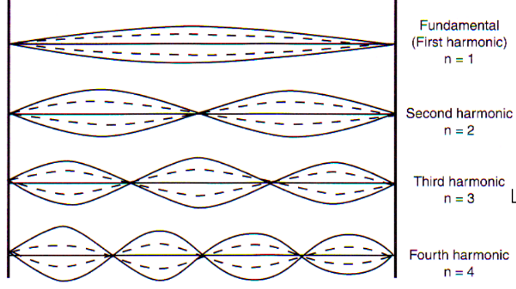
\includegraphics[width=0.6\textwidth, keepaspectratio]{harmonics.png}
        \label{fig:harmonics}
    \end{figure}

\begin{unprblm}[equação da onda unidimensional, primeiro harmônico]
    Considere a equação da onda unidimensional
    \begin{equation}
        u_{tt} = u_{xx}, \quad 0 < x < 1, \quad t > 0
    \end{equation} com condições de contorno e condições iniciais dadas por
    \begin{gather}
        u(0,t) = 0, \quad u(1,t) = 0, \quad t > 0 \\
        u(x,0) = \sin(\pi x), \quad u_t(x,0) = 0, \quad 0 < x < 1,
    \end{gather} e cuja solução exata é dada por
    \begin{equation} \label{eq:solucao_exata}
        u(x,t) = \sin(\pi x) \cos(\pi t), \quad 0 < x < 1, \quad t > 0
    \end{equation}
\end{unprblm}

\section{Metodologia}

Usamos o método explícito de diferenças finitas para resolver o problema numericamente. Construímos uma malha selecionando inteiros \(m\) e \(N\) que definem o número de subintervalos no espaço e no tempo, respectivamente. Fazendo \(h = l/m\) e \(k = T/N\), obtemos os pontos da malha \(x_i = i h\) para \(i = 0, 1, \ldots, m\) e \(t_j = j k\) para \(j = 0, 1, \ldots, N\). Em todo ponto interior da malha, a equação da onda se torna
\begin{equation}\label{eq:onda_discreta}
    \frac{\partial^2 u}{\partial t^2}(x_i, t_j) = \frac{\partial^2 u}{\partial x^2}(x_i, t_j), \quad 1 \leq i \leq m-1, \quad 1 \leq j \leq N-1.
\end{equation}

O método de diferenças finitas é obtido aproximando as derivadas de segunda ordem por diferenças centrais dadas por
\begin{equation}
    \frac{\partial^2 u}{\partial t^2} = \frac{u(x_i, t_{j+1}) - 2u(x_i, t_j) + u(x_i, t_{j-1})}{k^2} - \frac{k^2}{12} \frac{\partial^4 u}{\partial t^4}(x_i, \mu_j),
\end{equation} para algum \(\mu_j \in (t_{j-1}, t_{j+1})\), e
\begin{equation}
    \frac{\partial^2 u}{\partial x^2} = \frac{u(x_{i+1}, t_j) - 2u(x_i, t_j) + u(x_{i-1}, t_j)}{h^2} - \frac{h^2}{12} \frac{\partial^4 u}{\partial x^4}(\xi_i, t_j),
\end{equation} para algum \(\xi_i \in (x_{i-1}, x_{i+1})\). Substituindo essas aproximações na equação \eqref{eq:onda_discreta}, fica
\begin{multline} \label{eq:solucao_erro}
    \frac{u(x_i, t_{j+1}) - 2u(x_i, t_j) + u(x_i, t_{j-1})}{k^2} - \frac{u(x_{i+1}, t_j) - 2u(x_i, t_j) + u(x_{i-1}, t_j)}{h^2} \\
    = \frac{k^2}{12} \frac{\partial^4 u}{\partial t^4}(x_i, \mu_j) - \frac{h^2}{12} \frac{\partial^4 u}{\partial x^4}(\xi_i, t_j).
\end{multline} Negligenciado o termo de truncamento, obtemos a equação a diferenças
\begin{equation}
    \frac{w_{i, j+1} - 2w_{i, j} + w_{i, j-1}}{k^2} - \frac{w_{i+1, j} - 2w_{i, j} + w_{i-1, j}}{h^2} = 0.
\end{equation} Definindo \(\lambda = k/h\) e resolvendo para \(w_{i, j+1}\), a equação acima pode ser reescrita como
\begin{equation}\label{eq:solucao_diferencas_finitas}
    w_{i, j+1} = 2(1 - \lambda^2) w_{i, j} + \lambda^2 (w_{i+1, j} + w_{i-1, j}) - w_{i, j-1},
\end{equation} para \(i = 1, 2, \ldots, m-1\) e \(j = 1, 2, \ldots, N-1\). As condições de contorno e inicial são discretizadas como
\begin{gather}
    w_{0, j} = w_{m, j} = 0, \quad j = 1, 2, \ldots, N, \\
    w_{i, 0} = \sin(\pi x_i), \quad i = 1, 2, \ldots, m-1. 
\end{gather} Escrevendo em forma matricial, a equação a diferenças pode ser expressa como
\begin{equation}
    \begin{bmatrix}
        w_{1, j+1} \\
        w_{2, j+1} \\
        \vdots \\
        w_{m-1, j+1}
    \end{bmatrix} =
    \begin{bmatrix}
        2(1 - \lambda^2) & \lambda^2 & 0 & \cdots & 0 \\
        \lambda^2 & 2(1 - \lambda^2) & \lambda^2 & \cdots & 0 \\
        0 & \lambda^2 & 2(1 - \lambda^2) & \cdots & 0 \\
        \vdots & \vdots & \vdots & \ddots & \vdots \\
        0 & 0 & 0 & \cdots & 2(1 - \lambda^2)
    \end{bmatrix}
    \begin{bmatrix}
        w_{1, j} \\
        w_{2, j} \\
        \vdots \\
        w_{m-1, j}
    \end{bmatrix} -
    \begin{bmatrix}
        w_{1, j-1} \\
        w_{2, j-1} \\
        \vdots \\
        w_{m-1, j-1}
    \end{bmatrix}.
\end{equation} Notamos que para calcular \(w_{i, j+1}\) precisamos de \(w_{i, j}\) e \(w_{i, j-1}\). Isso significa que precisamos de duas condições iniciais para iniciar o processo de iteração. A primeira condição inicial é dada por \(w_{i, 0} = \sin(\pi x_i)\). Para obter a segunda condição inicial \(w_{i, 1}\), usamos a condição inicial da velocidade \(u_t(x,0) = 0\). Fazemos a expansão de \(u(x_i, t_1)\) em um polinômio de Maclaurin de segunda ordem em \(t\). Então
\begin{equation}
    u(x_i, t_1) = u(x_i, 0) + k \frac{\partial u}{\partial t}(x_i, 0) + \frac{k^2}{2} \frac{\partial^2 u}{\partial t^2}(x_i, 0) + \frac{k^3}{6} \frac{\partial^3 u}{\partial t^3}(x_i, \hat{\mu}_i),
\end{equation} para algum \(\hat{\mu}_i \in (0, t_1)\). Substituindo a equação da onda na equação acima, obtemos
\begin{equation}
    \frac{\partial^2 u}{\partial t^2}(x_i, 0) = \frac{\partial^2 u}{\partial x^2}(x_i, 0) = \frac{\partial^2}{\partial x^2} \sin(\pi x_i) = -\pi^2 \sin(\pi x_i),
\end{equation} e
\begin{equation}
    u(x_i, t_1) = \sin(\pi x_i) - \frac{k^2 \pi^2}{2} \sin(\pi x_i) + \frac{k^3}{6} \frac{\partial^3 u}{\partial t^3}(x_i, \hat{\mu}_i).
\end{equation} Isso nos dá a segunda condição inicial \(w_{i, 1}\) como
\begin{equation}
    w_{i, 1} = \sin(\pi x_i) - \frac{k^2 \pi^2}{2} \sin(\pi x_i).
\end{equation} Ainda, como \(\sin(\pi x) \in C^4[0,1]\), podemos aproximar a segunda derivada espacial \(\frac{\partial^2}{\partial x^2}\sin(\pi x_i)\) por diferenças centrais, obtendo
\begin{equation}
    w_{i, 1} = (1 - \lambda^2) w_{i, 0} + \frac{\lambda^2}{2} (w_{i+1, 0} + w_{i-1, 0}),
\end{equation} para \(i = 1, 2, \ldots, m-1\). A implementação numérica do método descrito acima é apresentada na Listagem \ref{lst:wave}.

\begin{lstlisting}[language=Python, caption={Função para resolver a equação da onda unidimensional usando diferenças finitas.}, label={lst:wave}]
    def wave(m, N, x_bounds, t_bounds, alpha, boundary, initial):
        """
        Solves the 1D wave equation using finite differences.

        Parameters
        ----------
        m : int
            Number of subintervals in the spatial direction.
        N : int
            Number of subintervals in the time direction.
        x_bounds : np.array
            An array defining the bounds of the spatial axis.
        t_bounds : np.array
            An array defining the bounds of the time axis.
        alpha : float
            The wave speed.
        boundary : dict
            A dictionary specifying the boundary conditions with keys 'left', 'right' and corresponding values for each boundary.
        initial : dict
            A dictionary specifying the initial conditions with keys 'u0' and 'u1' for the initial displacement and initial velocity, respectively.

        Returns
        -------
        w : 2D numpy array
            The solution to the wave equation on the grid defined by x_bounds and t_bounds.
        """
        import numpy as np

        # grid setup
        x_min, x_max = x_bounds[0], x_bounds[1]
        t_min, t_max = t_bounds[0], t_bounds[1]
        h = (x_max - x_min) / m
        k = (t_max - t_min) / N

        # create grid points
        x = np.linspace(x_min, x_max, m + 1)
        t = np.linspace(t_min, t_max, N + 1)

        # precompute constant for the update
        lmbda = (alpha * k / h)

        # initialize solution array
        w = np.zeros((m + 1, N + 1))

        # apply initial condition
        for i in range(m + 1):
            w[i, 0] = initial['u0'](x[i])

        # apply boundary conditions at all time steps
        w[0, :] = boundary['left']
        w[-1, :] = boundary['right']

        # compute the first time step using the initial derivative
        for i in range(1, m):
            w[i, 1] = (1 - lmbda**2) * w[i, 0] + (lmbda**2 / 2) * (w[i + 1, 0] + w[i - 1, 0]) + k * initial['u1'](x[i])

        # time-stepping loop for subsequent time steps
        for j in range(1, N):
            for i in range(1, m):
                w[i, j + 1] = (2 * (1 - lmbda**2) * w[i, j] + lmbda**2 * (w[i + 1, j] + w[i - 1, j]) - w[i, j - 1])

        return w
\end{lstlisting}

\section{Resultados e Conclusão}

Fazemos três experimentos com diferentes valores de \(\lambda\) para observar o comportamento da solução numérica. Os resultados são apresentados nas Figuras \ref{fig:wave_1}, \ref{fig:wave_2} e \ref{fig:wave_3} e nas Tabelas \ref{tab:resultados_lambda_1}, \ref{tab:resultados_lambda_0.2} e \ref{tab:resultados_lambda_1.2}.

Primeiro, estudamos o caso \(\lambda = 1\), com \(h = 0.1\) e \(k = 0.1\), que é o valor crítico para a estabilidade do método \cite{IK}. A Figura \ref{fig:wave_1} mostra a evolução temporal da solução numérica em comparação com a solução analítica. Observamos que a solução numérica aproxima muito bem com a solução analítica, indicando que o método é preciso e estável para este valor de \(\lambda\). Isso porque quando \(\lambda = 1\), a equação \eqref{eq:solucao_diferencas_finitas} se torna
\begin{equation}\label{eq:solucao_lambda1}
    w_{i, j+1} = w_{i+1, j} + w_{i-1, j} - w_{i, j-1},
\end{equation} o que coincide com a solução analítica \eqref{eq:solucao_exata}, pois
\begin{align}
    u(x, t) &= \sin(\pi x) \cos(\pi t) \\
    &= \frac{1}{2} \sin(\pi (x - t)) + \frac{1}{2} \sin(\pi (x + t))
\end{align} e a solução geral de d'Alembert é dada por \cite[134]{moyses_ondas}
\begin{equation}\label{eq:solucao_dalembert}
    u(x, t) = f(x - t) + g(x + t),
\end{equation} onde \(f\) e \(g\) são ondas viajando para a direita e para a esquerda, respectivamente. Resolvendo \eqref{eq:solucao_dalembert} para \(u(x, t + k)\), obtemos
\begin{align}
    u(x, t + k) &= f(x - (t + k)) + g(x + (t + k)) \\
    &= f((x - k) - t) + g((x + k) + t) \\
    &= u(x - k, t) + u(x + k, t) - u(x, t - k),
\end{align} que concorda com a equação \eqref{eq:solucao_lambda1}.

\begin{figure}[H]
    \centering
    \begin{subfigure}{0.48\textwidth}
        \centering
        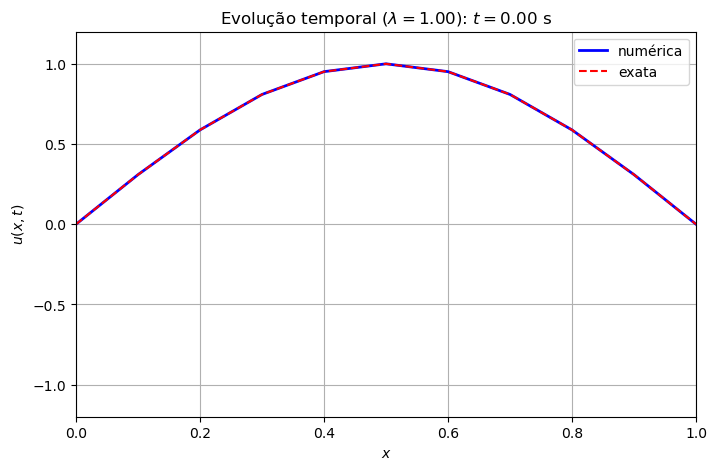
\includegraphics[width=\textwidth]{wave_1_t_0.00.png}
        \caption{$t = 0.00$ s}
        \label{fig:wave_1_t000}
    \end{subfigure}
    \hfill
    \begin{subfigure}{0.48\textwidth}
        \centering
        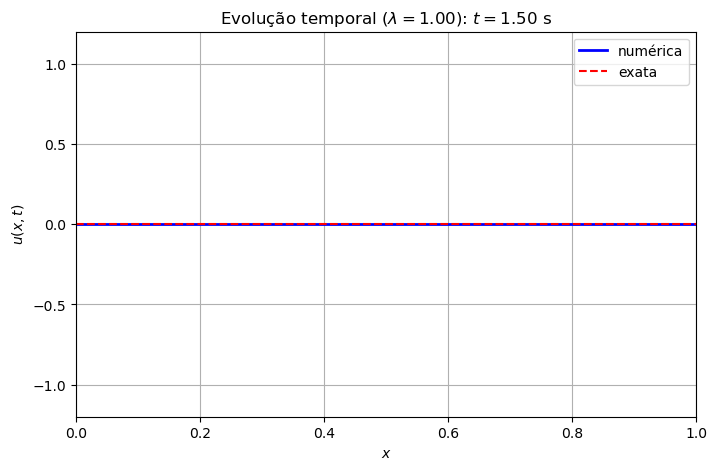
\includegraphics[width=\textwidth]{wave_1_t_1.50.png}
        \caption{$t = 1.50$ s}
        \label{fig:wave_1_t150}
    \end{subfigure}
    
    \vspace{0.3cm}
    
    \begin{subfigure}{0.48\textwidth}
        \centering
        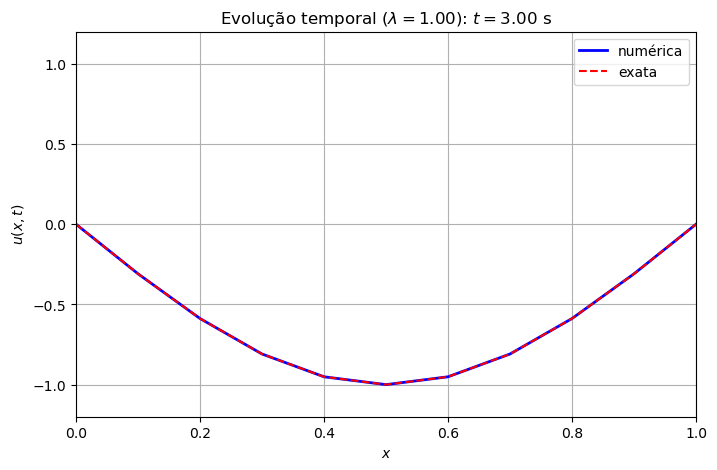
\includegraphics[width=\textwidth]{wave_1_t_3.00.png}
        \caption{$t = 3.00$ s}
        \label{fig:wave_1_t300}
    \end{subfigure}
    \hfill
    \begin{subfigure}{0.48\textwidth}
        \centering
        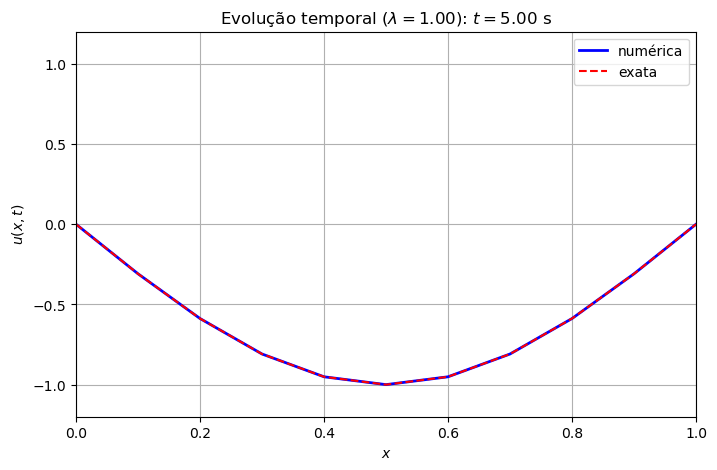
\includegraphics[width=\textwidth]{wave_1_t_5.00.png}
        \caption{$t = 5.00$ s}
        \label{fig:wave_1_t500}
    \end{subfigure}
    
    \caption{Evolução temporal do modo fundamental da equação da onda 1D com $\lambda = 1$. A linha azul representa a solução numérica por diferenças finitas e a linha tracejada vermelha representa a solução analítica.}
    \label{fig:wave_1}
\end{figure}

\begin{table}[H]
    \centering
    \caption{Resultados para \(\lambda = 1\)}
    \label{tab:resultados_lambda_1}
    \begin{tabular}{cccc}
        \toprule
        \(x_i\) & \(w_{i, 5}\) & \(u(x_i, 5)\) & \(|w_{i, 5} - u(x_i, 5)|\) \\
        \midrule
        0.0 & 0.00000000 & -0.00000000 & 0.0000e+00 \\
        0.1 & -0.30901699 & -0.30901699 & 5.5511e-17 \\
        0.2 & -0.58778525 & -0.58778525 & 1.1102e-16 \\
        0.3 & -0.80901699 & -0.80901699 & 0.0000e+00 \\
        0.4 & -0.95105652 & -0.95105652 & 5.5511e-16 \\
        0.5 & -1.00000000 & -1.00000000 & 0.0000e+00 \\
        0.6 & -0.95105652 & -0.95105652 & 4.4409e-16 \\
        0.7 & -0.80901699 & -0.80901699 & 0.0000e+00 \\
        0.8 & -0.58778525 & -0.58778525 & 5.5511e-16 \\
        0.9 & -0.30901699 & -0.30901699 & 5.5511e-17 \\
        \bottomrule
    \end{tabular}
\end{table}

Para o caso \(\lambda = 0.2\), com \(h = 0.1\) e \(k = 0.02\), o método também é estável, e é possível ver na Tabela \ref{tab:resultados_lambda_0.2} que o erro numérico coincide com o erro de truncamento \(\mathcal{O}(k^2 + h^2)\) visto em \eqref{eq:solucao_erro}.

\begin{figure}[H]
    \centering
    \begin{subfigure}{0.48\textwidth}
        \centering
        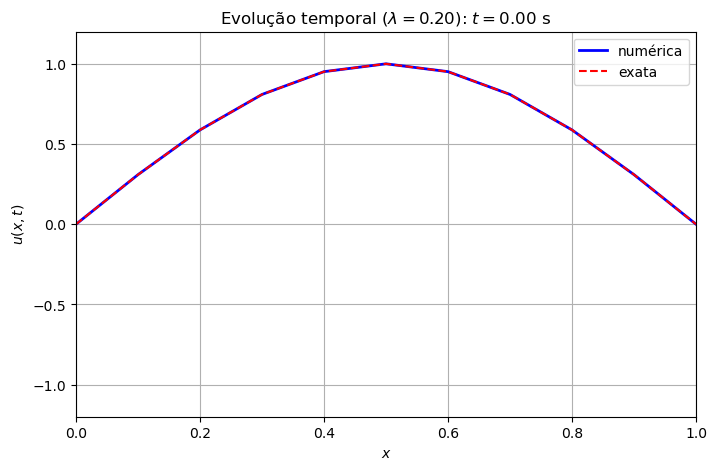
\includegraphics[width=\textwidth]{wave_2_t_0.00.png}
        \caption{$t = 0.00$ s}
        \label{fig:wave_2_t000}
    \end{subfigure}
    \hfill
    \begin{subfigure}{0.48\textwidth}
        \centering
        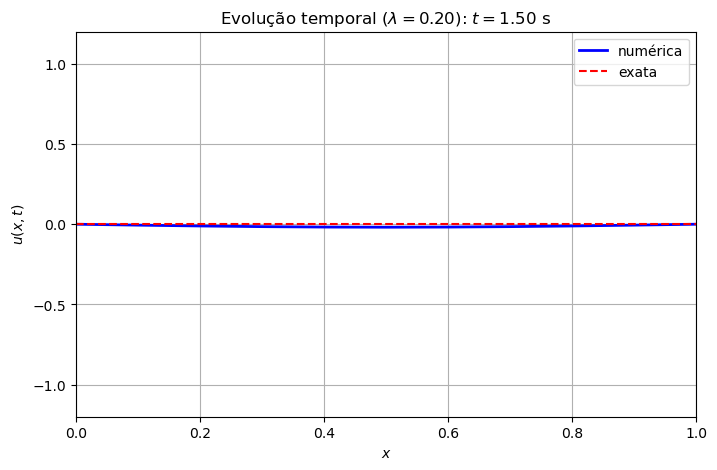
\includegraphics[width=\textwidth]{wave_2_t_1.50.png}
        \caption{$t = 1.50$ s}
        \label{fig:wave_2_t150}
    \end{subfigure}
    \vspace{0.3cm}
    \begin{subfigure}{0.48\textwidth}
        \centering
        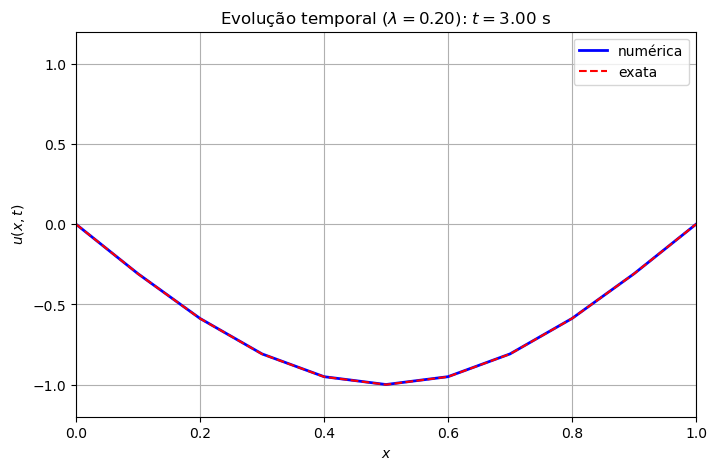
\includegraphics[width=\textwidth]{wave_2_t_3.00.png}
        \caption{$t = 3.00$ s}
        \label{fig:wave_2_t300}
    \end{subfigure}
    \hfill
    \begin{subfigure}{0.48\textwidth}
        \centering
        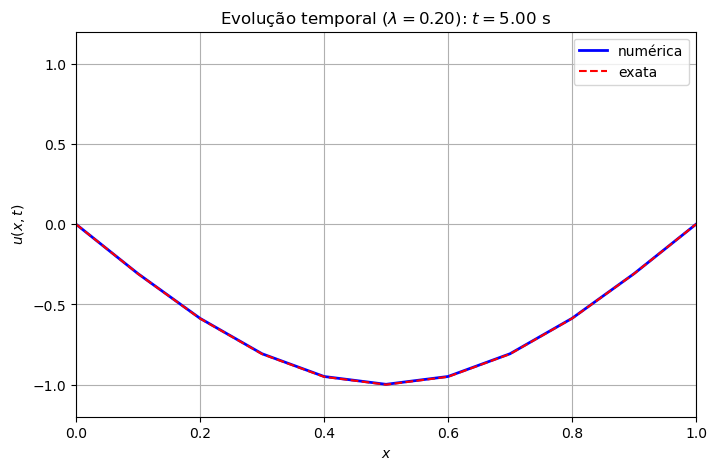
\includegraphics[width=\textwidth]{wave_2_t_5.00.png}
        \caption{$t = 5.00$ s}
        \label{fig:wave_2_t500}
    \end{subfigure}
    \caption{Evolução temporal do modo fundamental da equação da onda 1D com $\lambda = 0.2$.}
    \label{fig:wave_2}
\end{figure}

\begin{table}[H]
    \centering
    \caption{Resultados para \(\lambda = 0.2\)}
    \label{tab:resultados_lambda_0.2}
    \begin{tabular}{cccc}
        \toprule
        \(x_i\) & \(w_{i, 5}\) & \(u(x_i, 5)\) & \(|w_{i, 5} - u(x_i, 5)|\) \\
        \midrule
        0.0 & 0.00000000 & -0.00000000 & 0.0000e+00 \\
        0.1 & -0.30842395 & -0.30901699 & 5.9304e-04 \\
        0.2 & -0.58665722 & -0.58778525 & 1.1280e-03 \\
        0.3 & -0.80746439 & -0.80901699 & 1.5526e-03 \\
        0.4 & -0.94923132 & -0.95105652 & 1.8252e-03 \\
        0.5 & -0.99808088 & -1.00000000 & 1.9191e-03 \\
        0.6 & -0.94923132 & -0.95105652 & 1.8252e-03 \\
        0.7 & -0.80746439 & -0.80901699 & 1.5526e-03 \\
        0.8 & -0.58665722 & -0.58778525 & 1.1280e-03 \\
        0.9 & -0.30842395 & -0.30901699 & 5.9304e-04 \\
        \bottomrule
    \end{tabular}
\end{table}

Por fim, para o caso \(\lambda = 1.2\), com \(h = 0.1\) e \(k = 0.12\), o método não é estável, como é possível ver na Figura \ref{fig:wave_3_t500}. A Tabela \ref{tab:resultados_lambda_1.2} mostra que o erro numérico explode e se afasta da solução analítica, indicando que o método não converge para este valor de \(\lambda\). Esse resultado é consistente com a análise de estabilidade do método, que mostra que o método é estável apenas para \(\lambda \leq 1\) \cite[489]{IK}.

\begin{figure}[H]
    \centering
    \begin{subfigure}{0.48\textwidth}
        \centering
        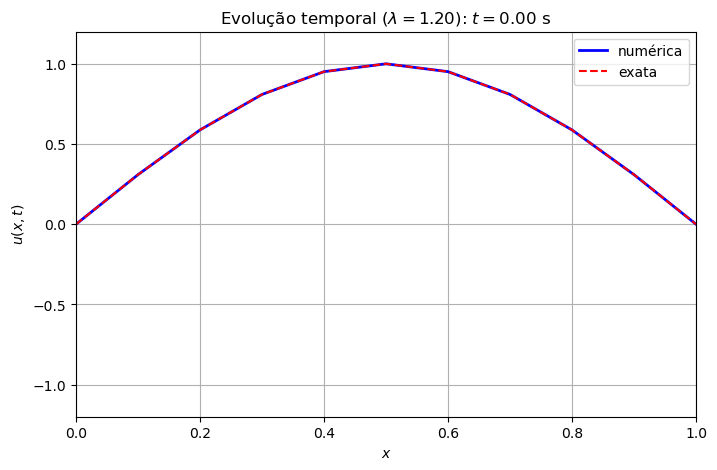
\includegraphics[width=\textwidth]{wave_3_t_0.00.png}
        \caption{$t = 0.00$ s}
        \label{fig:wave_3_t000}
    \end{subfigure}
    \hfill
    \begin{subfigure}{0.48\textwidth}
        \centering
        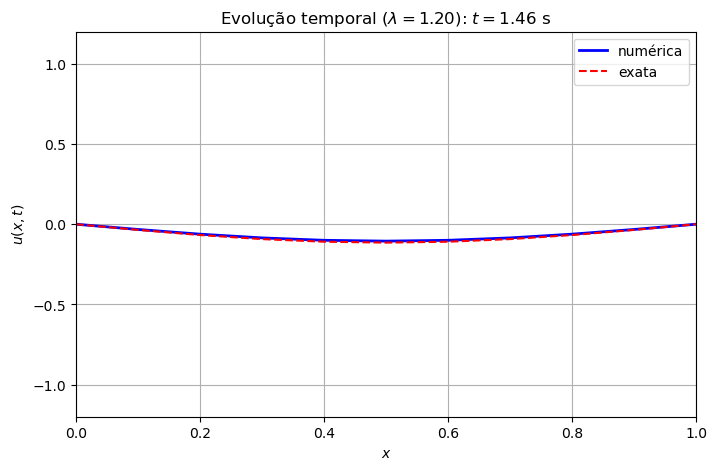
\includegraphics[width=\textwidth]{wave_3_t_1.46.png}
        \caption{$t = 1.46$ s}
        \label{fig:wave_3_t146}
    \end{subfigure}
    \vspace{0.3cm}
    \begin{subfigure}{0.48\textwidth}
        \centering
        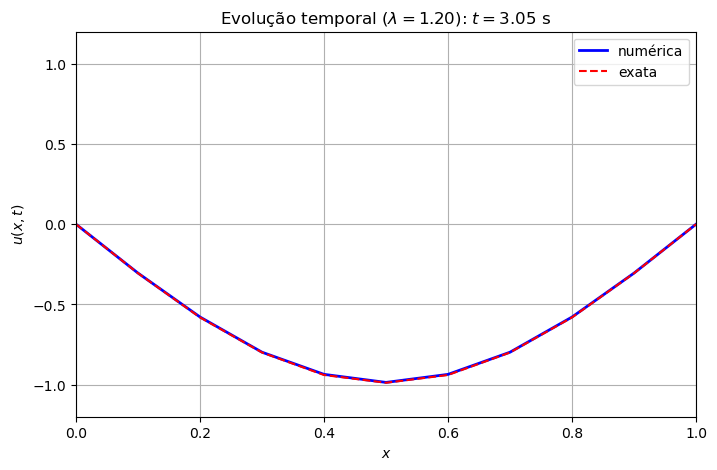
\includegraphics[width=\textwidth]{wave_3_t_3.05.png}
        \caption{$t = 3.05$ s}
        \label{fig:wave_3_t305}
    \end{subfigure}
    \hfill
    \begin{subfigure}{0.48\textwidth}
        \centering
        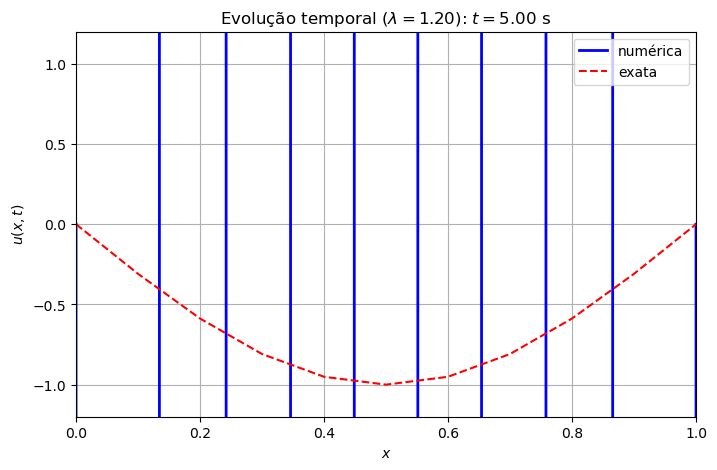
\includegraphics[width=\textwidth]{wave_3_t_5.00.png}
        \caption{$t = 5.00$ s}
        \label{fig:wave_3_t500}
    \end{subfigure}
    \caption{Evolução temporal do modo fundamental da equação da onda 1D com $\lambda = 1.2$.}
    \label{fig:wave_3}
\end{figure}

\begin{table}[H]
    \centering
    \caption{Resultados para \(\lambda = 1.2\)}
    \label{tab:resultados_lambda_1.2}
    \begin{tabular}{cccc}
        \toprule
        \(x_i\) & \(w_{i, 5}\) & \(u(x_i, 5)\) & \(|w_{i, 5} - u(x_i, 5)|\) \\
        \midrule
        0.0 & 0.00000000 & -0.00000000 & 0.0000e+00 \\
        0.1 & -173015.37874265 & -0.30901699 & 1.7302e+05 \\
        0.2 & 328811.25437226 & -0.58778525 & 3.2881e+05 \\
        0.3 & -451966.12936866 & -0.80901699 & 4.5197e+05 \\
        0.4 & 530419.43046658 & -0.95105652 & 5.3042e+05 \\
        0.5 & -556672.80998304 & -1.00000000 & 5.5667e+05 \\
        0.6 & 528431.36623167 & -0.95105652 & 5.2843e+05 \\
        0.7 & -448749.37386477 & -0.80901699 & 4.4875e+05 \\
        0.8 & 325594.49886836 & -0.58778525 & 3.2560e+05 \\
        0.9 & -171027.31450774 & -0.30901699 & 1.7103e+05 \\
        \bottomrule
    \end{tabular}
\end{table}


\printbibliography


\end{document}